\chapter{Практическая часть}
\label{ch:chap2}

\section*{Adalm Pluto SDR}

\textbf{Adalm Pluto SDR} - модель SDR, разработанная компанией \textbf{Analog Devices} для обучения основам SDR.

\begin{figure}[H]
    \centering
    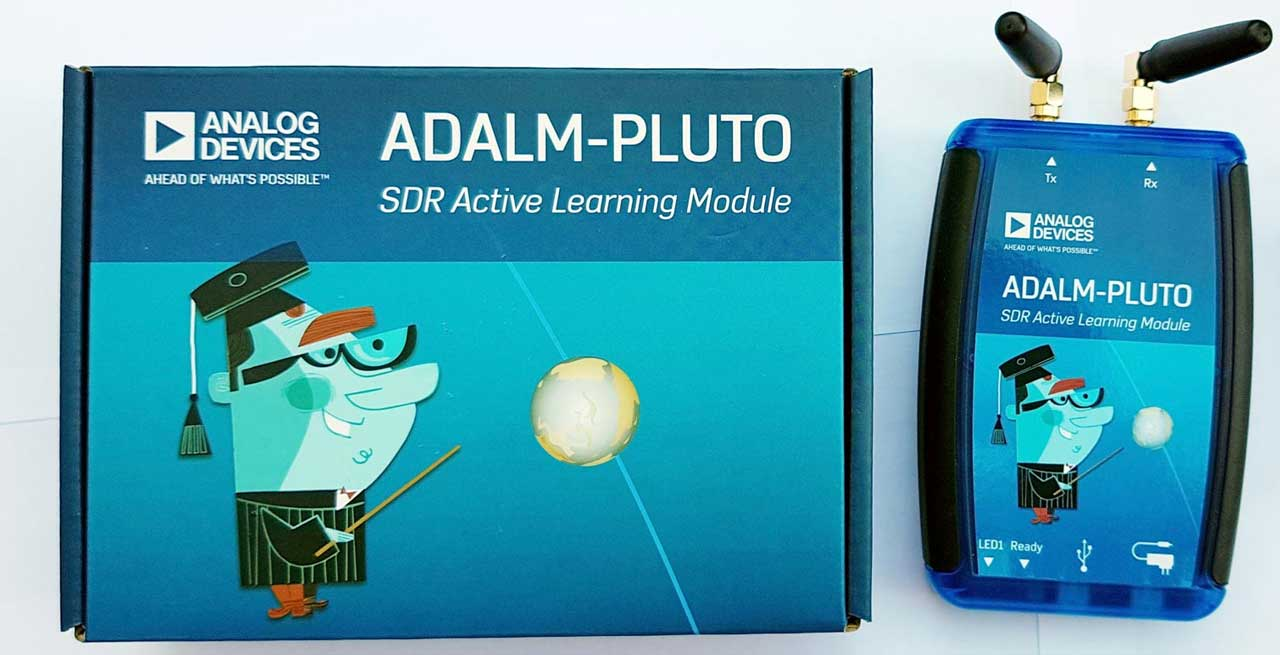
\includegraphics[width=0.8\textwidth]{AdalmPluto.png}
    \caption{Внешний вид Adalm Pluto}
\end{figure}

\section*{Архитектура Adalm Pluto SDR}

\begin{figure}[H]
    \centering
    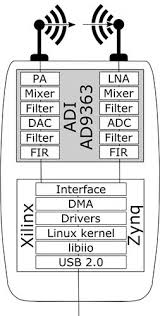
\includegraphics[width=0.6\textwidth]{AdalmArch.png}
    \caption{Архитектура Adalm Pluto}
\end{figure}

\section*{Описание основных блоков Adalm Pluto}

\subsection*{\textbf{PA (Power Amplifier)}}
\begin{description}
  \item[\textbf{Функция:}] Усиление сигнала.
\end{description}

\subsection*{\textbf{LNA (Low Noise Amplifier)}}
\begin{description}
  \item[\textbf{Функция:}] Усиление слабого приёмного сигнала с минимальным добавлением шума.
\end{description}

\subsection*{\textbf{ADC / DAC}}
\begin{description}
  \item[\textbf{ADC (Analog-to-Digital Conversion):}] оцифровка аналогового сигнала.
  \item[\textbf{DAC (Digital-to-Analog Conversion):}] преобразование цифровых семплов в аналоговый сигнал.
\end{description}

\subsection*{\textbf{FIR (Finite Impulse Response)}}
\begin{description}
  \item[\textbf{Функция:}] детальная фильтрация, коррекция формы спектра.
\end{description}

\subsection*{\textbf{Mixer}}
\begin{description}
  \item[\textbf{TX:}] перенос низкочастотного сигнала на несущую частоту.
  \item[\textbf{RX:}] перенос высокочастотного сигнала на низкочастотный.
\end{description}

\subsection*{\textbf{Filter}}
\begin{description}
  \item[\textbf{TX:}] фильтрация выходного сигнала перед передачей.
  \item[\textbf{RX:}] фильтрация принимаемого сигнала.
\end{description}

\subsection*{\textbf{libiio}}
\begin{description}
  \item[\textbf{Описание:}] библиотека, которая облегчает работу с устройствами ввода/вывода в \textbf{Linux}. 
  Она даёт \textbf{API} для обмена данными и управления устройствами.
\end{description}

\subsection*{\textbf{Linux Kernel}}
\begin{description}
  \item[\textbf{Описание:}] ядро \textbf{Linux}. Управляет железом.
\end{description}

\subsection*{\textbf{Drivers}}
\begin{description}
  \item[\textbf{Описание:}] обеспечение корректной работы Linux с устройствами.
\end{description}

\subsection*{\textbf{Xilinx Zynq}}
\begin{description}
  \item[\textbf{Описание:}] семейство микросхем от компании Xilinx. На одном кристалле 
  объединены ARM-процессор, на котором работает Linux, и ПЛИС для более скоростных вычислений. 
\end{description}


\subsection*{\textbf{GNU Radio}}

\begin{figure}[H]
    \centering
    
\includegraphics[width=1.0\textwidth]{GNURadio.png}
    \caption{Логотип GNU Radio}
\end{figure}

\textbf{GNU Radio} - это инструмент с открытым исходным кодом для разработки программного обеспечения 
в сфере программно-определяемого радио. 

Он позволяет при помощи «строительных блоков» создавать конфигурации радиоустройств, не написав ни одной строчки кода, 
и запускать программы непосредственно с использованием SDR-модулей, например: \textbf{Adalm-Pluto}, \textbf{LimeSDR} и др. \\

В библиотеке имеется широкий спектр функций для цифровой обработки сигналов. Модули написаны на \textbf{C++}, 
а их взаимодействие реализовано на \textbf{Python}. Приложения можно строить как через \textbf{API GNU Radio}, 
так и посредством графического интерфейса \textbf{GNU Radio Companion (GRC)}.

\section*{\textbf{Построение схемы в GNU Radio}}

\subsection*{\textbf{Блок options}}

\begin{figure}[H]
    \centering
    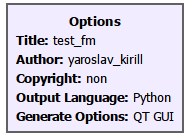
\includegraphics[width=0.5\textwidth]{options.png}
    \caption{Блок options}
\end{figure}

Этот блок задает настройки проекта. Самое важное здесь: \textbf{Output Language} и \textbf{Generate Options}. \\
\textbf{Output Language} — язык, на котором будет сгенерирован код программы. \\
\textbf{Generate Options} — используемый графический интерфейс.

\subsection*{\textbf{Блок variable}}

\begin{figure}[H]
    \centering
    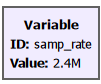
\includegraphics[width=0.5\textwidth]{var.png}
    \caption{Блок variable}
\end{figure}

В этом блоке можно задать переменную (почти как в языке программирования). Переменная имеет ID (имя) и значение.  
Здесь задается \texttt{samp\_rate} (частота дискретизации), равная $2.4 \times 10^6$ Hz.

\subsection*{\textbf{QT GUI Range}}

\begin{figure}[H]
    \centering
    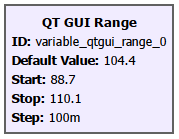
\includegraphics[width=0.5\textwidth]{qt_range.png}
    \caption{Блок QT GUI Range}
\end{figure}

Этот блок задает ползунок из QT, позволяющий удобно менять значение переменной во время работы программы.  
Это позволяет не перезапускать программу, когда нам требуется поменять какое-либо значение.  
Здесь задается ползунок для настройки частоты приема FM волны.

Основные параметры блока: 

\begin{itemize}
    \item \textbf{Default Value} — значение, которое будет устанавливаться при запуске программы;
    \item \textbf{Start} — минимальное значение;
    \item \textbf{Stop} — максимальное значение;
    \item \textbf{Step} — шаг изменения при сдвиге ползунка.
\end{itemize}

\subsection*{\textbf{PlutoSDR Source}}

\begin{figure}[H]
    \centering
    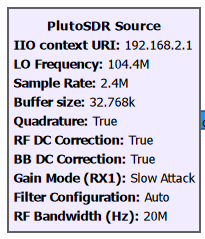
\includegraphics[width=0.5\textwidth]{source.png}
    \caption{Блок PlutoSDR Source}
\end{figure}

Этот блок отвечает за приём данных от устройства ADALM-Pluto (PlutoSDR). Он подключается к SDR, управляет настройками, получает поток отсчётов. \\

\textbf{Параметры:}

\begin{itemize}
    \item \textbf{IIO context URI} — IP адрес Adalm Pluto, нужен, потому что PlutoSDR может подключаться по USB или сети (Ethernet/USB-Ethernet);
    \item \textbf{Sample Rate} — частота дискретизации АЦП внутри PlutoSDR. Определяет, с какой частотой будут делаться отсчеты при оцифровке;
    \item \textbf{Buffer Size} — встроенный буфер для временного хранения данных перед их передачей в компьютер;
    \item \textbf{Quadrature} — задаём представление сигнала в виде I/Q семплов;
\end{itemize}

\subsection*{\textbf{Low Pass Filter}}

\begin{figure}[H]
    \centering
    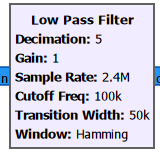
\includegraphics[width=0.5\textwidth]{filter.png}
    \caption{Блок Low Pass Filter}
\end{figure}

Ограничивает полосу сигнала, выделяя только FM-станцию. \\

\textbf{Параметры:}

\begin{itemize}
    \item \textbf{Decimation} — снижение частоты дискретизации в n раз;
    \item \textbf{Gain} — усиление амплитуды после фильтрации;
    \item \textbf{Sample Rate} — дефолтная частота дискретизации;
    \item \textbf{Cutoff Freq} — полоса 100 кГц (ширина FM сигнала).
\end{itemize}

\subsection*{\textbf{QT GUI Frequency Sink}}

\begin{figure}[H]
    \centering
    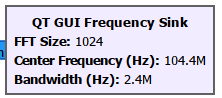
\includegraphics[width=0.5\textwidth]{freq_sink.png}
    \caption{Блок QT GUI Frequency Sink}
\end{figure}

Этот блок при помощи QT задает спектральное представление сигнала, которое меняется в реальном времени.  
Таких блоков 2: до фильтра (напрямую из блока source) и после фильтра. Первый показывает весь эфир, а второй — захваченный сигнал (именно FM частоту). \\

\textbf{Параметры:}

\begin{itemize}
    \item \textbf{FFT Size} — кол-во точек для спектра;
    \item \textbf{Center Frequency} — центральная частота захвата;
    \item \textbf{Bandwidth} — полоса частот захвата.
\end{itemize}

\subsection*{\textbf{QT GUI Time Sink}}

\begin{figure}[H]
    \centering
    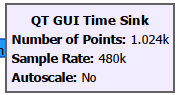
\includegraphics[width=0.5\textwidth]{time_sink.png}
    \caption{Блок QT GUI Time Sink}
\end{figure}

Этот блок при помощи QT задает временное представление сигнала, которое меняется в реальном времени. \\

\textbf{Параметры:}

\begin{itemize}
    \item \textbf{Number of Points} — кол-во точек, отображаемых в каждый момент времени;
    \item \textbf{Sample Rate} — частота дискретизации при отрисовке;
    \item \textbf{Autoscale} — нужно ли масштабировать сигнал по вертикали.
\end{itemize}

\subsection*{\textbf{WBFM Receive}}

\begin{figure}[H]
    \centering
    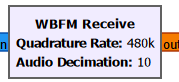
\includegraphics[width=0.5\textwidth]{wbfm.png}
    \caption{Блок WBFM Receive}
\end{figure}

Блок демодуляции FM-сигнала. \\

\textbf{Параметры:}

\begin{itemize}
    \item \textbf{Quadrature Rate} — входная частота дискретизации (после фильтра и децимации);
    \item \textbf{Audio Decimation} — уменьшение дискретизации для звука (в моем случае до 48k, чего вполне достаточно для звука).
\end{itemize}

На выходе — звуковой сигнал.

\subsection*{\textbf{Audio Sink}}

\begin{figure}[H]
    \centering
    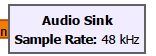
\includegraphics[width=0.5\textwidth]{audio_out.png}
    \caption{Блок Audio Sink}
\end{figure}

От \textbf{WBFM Receive} звук идет на блок \textbf{Audio Sink} — блок, который выводит звуковой поток на аудиокарту хоста. \\

\textbf{Параметры:}

\begin{itemize}
    \item \textbf{Sample Rate} — стандартная частота звука.
\end{itemize}

Соединить блоки нужно следующим образом, тогда у нас получится работающая радиосистема, которая будет принимать FM радио.

\begin{figure}[H]
    \centering
    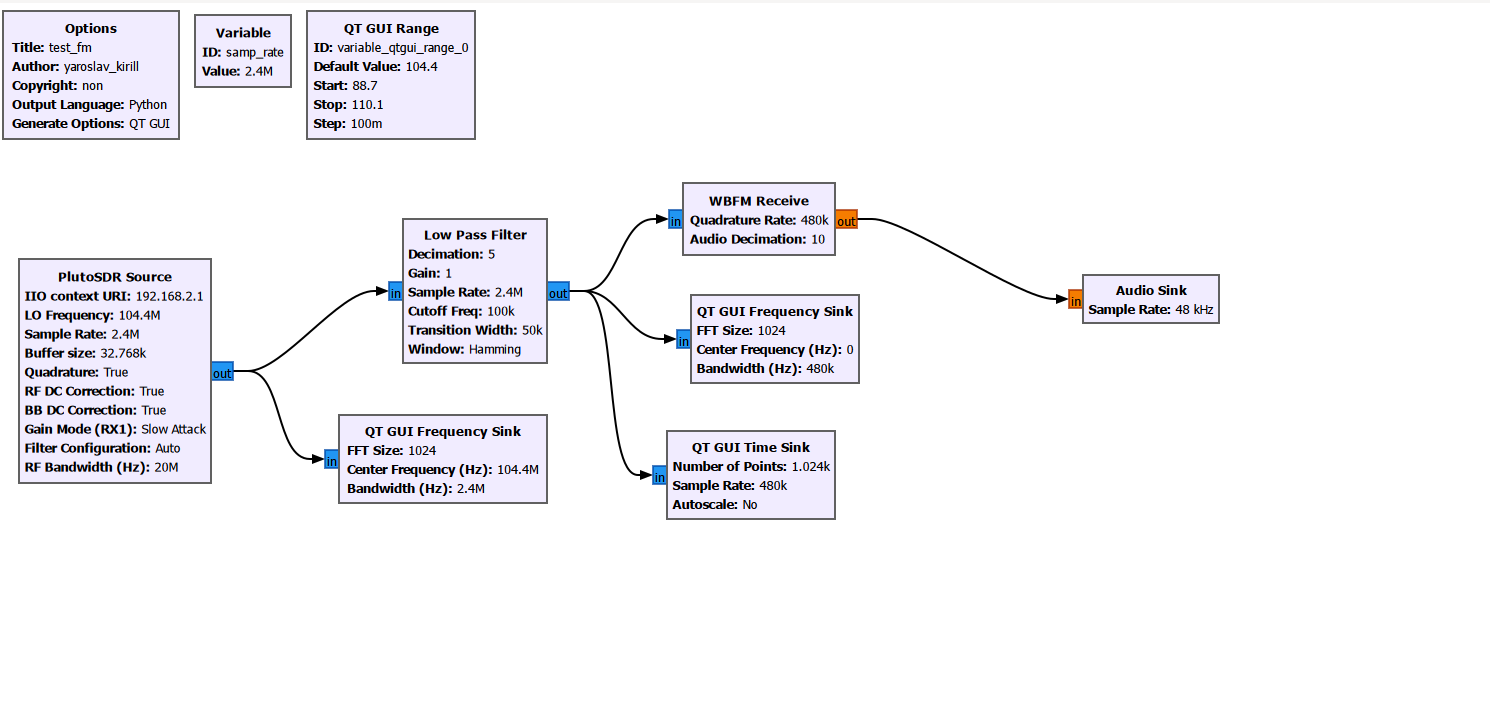
\includegraphics[width=1.0\textwidth]{system.png}
    \caption{Пример простой радиосистемы в GNURadio}
\end{figure}

\begin{figure}[H]
    \centering
    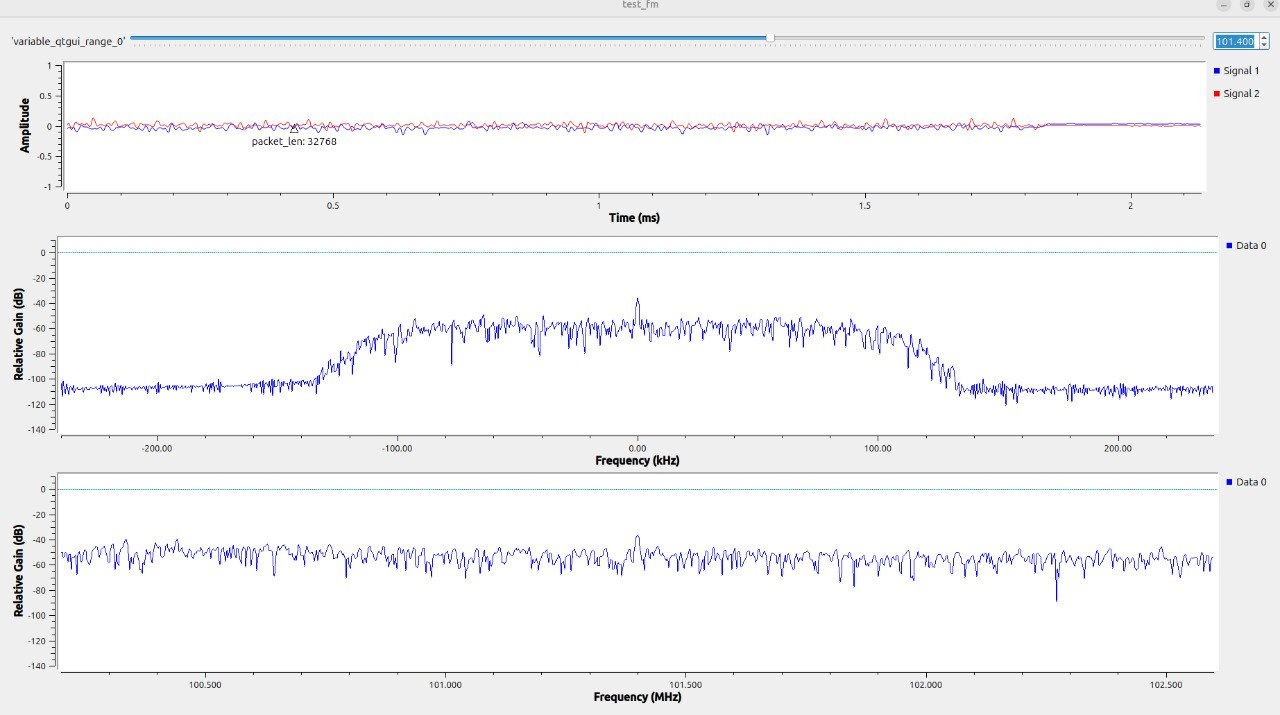
\includegraphics[width=1.0\textwidth]{gnuwork.png}
    \caption{Пример работы программы}
\end{figure}
